%
% teil1.tex -- Beispiel-File für das Paper
%
% (c) 2020 Prof Dr Andreas Müller, Hochschule Rapperswil
%
% !TEX root = ../../buch.tex
% !TEX encoding = UTF-8
%
\section{Lineares Medium\label{particles:section:linear}}
\kopfrechts{Lineares Medium}
% TODO: Quellenangaben
% [ ]: https://en.wikipedia.org/wiki/Linearity
% [ ]: Lineare Algebra: Eine anwendungsorientierte Einführung, Seite: 27, ISBN: 978-3-662-67865-7, Published: 01 September 2023, DOI: https://doi.org/10.1007/978-3-662-67866-4

\subsection{Was ist Linearität?}
Für den einfachsten und üblichsten Fall, nimmt man oft ein \emph{lineares Medium} an.
Solch ein Medium nennt man \emph{linear}, wenn dessen Definition sowohl \emph{additiv}
\[
    f(x_{1} + y_{1}, \ldots, x_{n} + y_{n}) 
    = 
    f(x_{1}, \ldots, x_{n}) 
    + 
    f(y_{1}, \ldots, y_{n}),
\]
als auch \emph{homogen}
\[
    f(\lambda x_{1}, \ldots, \lambda x_{n}) 
    = 
    \lambda f(x_{1}, \ldots, x_{n})
\]
ist.
Hierbei ist angemerkt, dass $x_{k}$, $y_{k}$ und $\lambda$ nicht rein reell sein müssen, 
sondern einem beliebigen Vektorraum angehören können, 
was für den zweidimensionalen Fall wichtig ist.

In der Wellentheorie bedeutet dies, 
dass die Materialeigenschaften---beispielsweise die Elastizität---nicht von der Amplitude der Welle abhängen.
Diese Elastizität eines Mediums lässt sich durch das \emph{hookesche Gesetz}
\[
    \Delta l
    = 
    \frac{F}{D}
    \quad
    \left(D = \text{const.} 
    \Rightarrow 
    \frac{\partial D}{\partial F} 
    \overset{!}{=} 
    0 
    \quad 
    \forall F \right)
    \label{particles:eq:hookesches-gesetz},
\]
welches bereits in abschnitt \mytodo{Verweis Elastizitätstheorie} verwendet wurde, beschreiben.
Dabei beschreibt $\Delta l$ die Distanzänderung zweier Punkte,
$F$ die dazwischen wirkende Kraft und $D$ einen Proportionalitätsfaktor.
Mittels Substitution kann man nun darauf schliessen, 
dass es sich hierbei tatsächlich um eine lineare Funktion handeln muss.

\begin{figure}
    \centering
    \subfigure[]{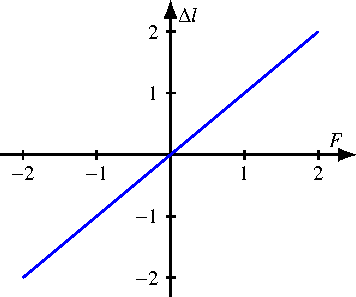
\includegraphics{./papers/particles/figures/out/lineares_medium_deformation.pdf}\label{particles:fig:lin-medium:deform}}\hfill
    \subfigure[]{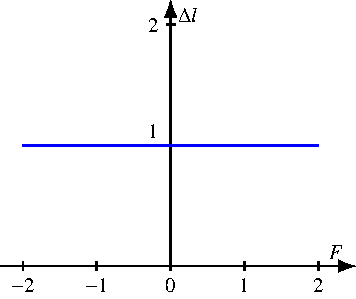
\includegraphics{./papers/particles/figures/out/lineares_medium_elast_modul.pdf}\label{particles:fig:lin-medium:elast-modul}}
    \caption{Deformation~(a) und Elastisches Modul~(b) eines linearen Mediums mit konstantem Faktor $D = 1$.}
\end{figure}

\subsection{Superpositionsprinzip}\label{particles:section:lin-medium:superposition}
Das Superpositionsprinzip fasst die Bedingungen zur Linearität nochmal etwas schöner in eine Formel zusammen, 
nämlich
\[
    T(\lambda x + \mu y)
    = 
    \lambda T(x) 
    + 
    \mu T(y).
\]
Blickt man wieder auf die Wellentheorie, so bedeutet dies, dass sich Wellen in linearen Medien überlagern, sich aber nicht gegenseitig beeinflussen.
Dies kann man schön anhand zweier sich kreuzende Laserstrahlen im Vakuum veranschaulichen, 
wie sie in Abbildung \mytodo{Abbildung zweier Laserstrahlen, die sich kreuzen, lokal interferieren, jedoch den weiteren Verlauf nicht verändern.} gezeigt werden.
Lokal interferieren diese Laserstrahlen zwar, stören jedoch nicht ihren weiteren Verlauf. 

\mytodo{Irgendwo sollte man noch ein Beispiel mit $E$- oder $B$-Feld einbringen}


\subsection{Schwinger-Limit}\label{particles:section:lin-medium:schwinger}
Bei extrem hohen Feldstärken tritt ein Phänomen auf, wobei das Vakuum selbst nichtlinear wird.
Dieser Übergang zur Nichtlinearität des Vakuums nennt man das \emph{Schwinger-Limit}\mytodo{Quellenangabe}, benannt nach Julian Schwinger, welcher 1951 dieses Phänomen erstmals theoretisierte.
Da es sich hierbei um elektrische und magnetische Feldstärken im Bereich von $10^{18}\,\frac{\text{V}}{\text{m}}$ und $10^9\,\text{T}$ handelt, konnte dieses Limit bisher noch nicht konkret nachgewiesen oder gemessen werden.
Es ist entsprechend noch immer Bestandteil aktueller Forschungen. \mytodo{Quelle hierfür angeben}

Beschränkt man sich jedoch nicht nur auf das Vakuum, so findet man Medien, welche bereits bei deutlich kleineren Feldstärken nichtlineare Eigenschaften aufweisen.
Ein Beispiel von solchen nichtlinearen Werkstoffen sind, wie~\ref{particles:frequenzverdopplung} demonstriert, Kristalle zur Frequenzverdoppelung.
Diese werden zum Beispiel in grünen Laserpointern eingesetzt, was die Verwendung von preiswerteren Infrarot-Laserdioden anstelle der teureren grünen Ausführung erlaubt.
